\documentclass[12pt,french,twoside]{report}
%%%%%%%%%%%%%%%%%%%%%%%%%%%%%%%%%%%%%%%%%%%%%%%%%%%%%%%%%%%%%%%%%%%%%%%%%%%%%%%
\usepackage{etex}
\usepackage[utf8x]{inputenc}
\usepackage[T1]{fontenc}
\usepackage{babel}
\usepackage{frcursive} % Pour l'écriture cursive
\usepackage[upright]{fourier}
\usepackage[scaled=0.875]{helvet}
\usepackage[dvipsnames,table]{xcolor}
\usepackage{fancyhdr}
%___________________________
%===    Numérotation
%------------------------------------------------------
\usepackage{enumerate} %permet la modif de la numérotation et de poursuivre une numérotation en cours avec \begin{enumerate}[resume]
\usepackage{enumitem}
\frenchbsetup{StandardLists=true}%frenchb ne s'occupera pas des listes
\setenumerate[1]{font=\bfseries,label=\arabic*.} % numérotation 1. 2. ...
\setenumerate[2]{font=\bfseries,label=\alph*)} % sous-numérotation a) b) ...
\usepackage{lastpage} % permet d'afficher le nombre total de pages après DEUX compilations.
%___________________________
%===    Pour les mathématiques
%------------------------------------------------------
%les commandes suivantes évitent le message "too many math alphabets"...
\newcommand\hmmax{0}
\newcommand\bmmax{0}
\usepackage{amssymb,mathtools}%symbole parallèle avec \sslash
\usepackage{bm} % pour l'écriture en gras des formules mathématiques avec \bm
\usepackage{cancel} % pour les simplifications de fractions
\renewcommand\CancelColor{\color{red}}
\usepackage[autolanguage,np]{numprint}
\DecimalMathComma %supprime l'espace après la virgule dans un nombre
\usepackage{dsfont} %écriture des ensemble N, R, C ...avec \mathds{}
\usepackage{mathrsfs}   % Police de maths jolie caligraphie \mathscr{}
%simplification de la notation de vecteur \vect{}
\newcommand{\vect}[1]{\mathchoice%
{\overrightarrow{\displaystyle\mathstrut#1\,\,}}%
{\overrightarrow{\textstyle\mathstrut#1\,\,}}%
{\overrightarrow{\scriptstyle\mathstrut#1\,\,}}%
{\overrightarrow{\scriptscriptstyle\mathstrut#1\,\,}}}
%Repères
\def\Oij{$\left(\text{O}\pv\vect{\imath},~\vect{\jmath}\right)$\xspace}
\def\Oijk{$\left(\text{O}\pv\vect{\imath},~ \vect{\jmath},~ \vect{k}\right)$\xspace}
\def\Ouv{$\left(\text{O}\pv\vect{u},~\vect{v}\right)$\xspace}
\def\OIJ{$\left(O\pv I\:,\,J\right)$\xspace}
%commandes perso
\newcommand\abs[1]{\ensuremath{\left\vert #1 \right\vert}}%valeur absolue
\newcommand\Arc[1]{\ensuremath{\wideparen{#1}}}%arc de cercle
%TikZ et TkZ
\usepackage{pgf,tikz,tkz-base,tkz-euclide,tkz-tab}
\usetkzobj{all}
%___________________________
%===    Pour les tableaux
%------------------------------------------------------
\usepackage{array}
\usepackage{longtable}
\usepackage{tabularx,tabulary}
\usepackage{multirow}
\usepackage{multicol}
\setlength\columnseprule{0.4pt}
\renewcommand{\arraystretch}{1.5}
\newcolumntype{M}[1]{>{\centering\arraybackslash}m{#1}}%cellule centrée horizontalement et verticalement


\usepackage{setspace}%INTERLIGNES
\usepackage{fancybox} % par exemple \ovalbox{}

\usepackage{pifont}
%checked box
\newcommand{\checkbox}{
\makebox[0pt][l]{$\square$}\raisebox{.15ex}{\hspace{0.1em}$\checkmark$}
}

\usepackage{pas-algo}%package de Stéphane Pasquet
\usepackage{pas-tableur}%package de Stéphane Pasquet
%___________________________
%===    Format de la page
%------------------------------------------------------
\setlength\paperheight{297mm}
\setlength\paperwidth{210mm}
\setlength{\textheight}{23,5cm}
% 
\usepackage{geometry}
\geometry{hmargin=2cm,vmargin=2.5cm,lmargin=1.5cm,rmargin=1.5cm}

%___________________________
%===    Entête du devoir uniquement sur la première page
%------------------------------------------------------
\fancypagestyle{garde_controle}{% 
\fancyhead[L]{\textbf{CNED}}
\fancyhead[R]{\textbf{1\up{ère} S}}
\renewcommand{\headrulewidth}{0cm}}

\newcommand{\controle}{
\noindent
\thispagestyle{garde_controle}
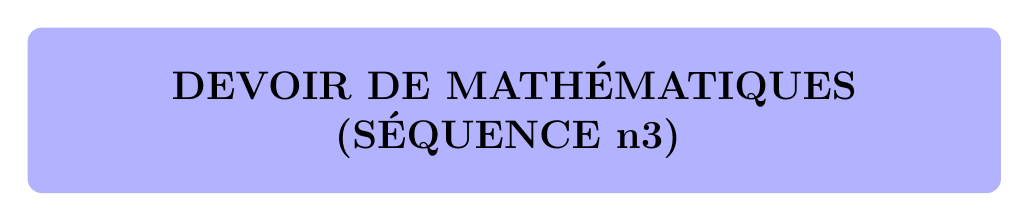
\begin{tikzpicture}[node distance=0 cm]
\node[fill=blue!30,rectangle,rounded corners=5pt]
{%
\begin{minipage}{\textwidth}
\begin{center}
\vspace*{9pt}
\Large \textsc{\textbf{DEVOIR DE MATH\'EMATIQUES (S\'EQUENCE n\degres 3)}}
\vspace*{9pt}
\end{center}
\end{minipage}
};
\end{tikzpicture}

\begin{center}
\begin{minipage}{0.8\linewidth}
\begin{center}
\textbf{À renvoyer à la correction.}

\textbf{Veuillez rédiger vos réponses aux exercices de ce devoir après avoir étudié la séquence n\degres 3.}
\end{center}
\end{minipage}
\end{center}
\noindent
}
%%%%%%%%%%%%%%%%%%%%%%%
%% DEBUT DU DOCUMENT %%
%%%%%%%%%%%%%%%%%%%%%%%

\begin{document}
\selectlanguage{french}
%\selectlanguage{english}
\controle

\setlength\parindent{0mm}
\pagestyle{fancy}
\fancyhf{}
\renewcommand \headrulewidth{0pt}%
\renewcommand \footrulewidth{0.2pt}%
\fancyfoot[L]{1\up{ère} S} 
\fancyfoot[C]{\thepage / \pageref{LastPage}} 
\fancyfoot[R]{Année 2016-2017}

%%%%%%%%%%%%%%%%%%%%%%%%%%%%%%%%%%%%%%%%%%%%%%%%%%%%%%%%%%%%%%%%%%%%%%%%%
\begin{spacing}{1.2}
%%%%%%%%%%%%%%%%%%%%%%%%%%%%%%%%%%%%%%%%%%%%%%%%%%%%%%%%%%%%%%%%%%%%%%%%%
%%%%%%%%%%%%%%%%%%%%%%%%%%%%%%%%%%%%%%%%%%%%%%%%%%%%%%%%%%%%%%%%%%%%%%%%%
%%%%%%%%%%%%%%%%%%%%%%%% exercice 1 %%%%%%%%%%%%%%%%%%%%%%%%%%%%%%%%%%%%%
%%%%%%%%%%%%%%%%%%%%%%%%%%%%%%%%%%%%%%%%%%%%%%%%%%%%%%%%%%%%%%%%%%%%%%%%%
\textbf{\large{Exercice 1 :}}\hfill \textbf{(\dots points)}
\medskip


\begin{center}
$\star\star\star\star\star\star\star\star\star\star\star\star\star\star$
\end{center}
%%%%%%%%%%%%%%%%%%%%%%%%%%%%%%%%%%%%%%%%%%%%%%%%%%%%%%%%%%%%%%%%%%%%%%%%%
%%%%%%%%%%%%%%%%%%%%%%%% exercice 2 %%%%%%%%%%%%%%%%%%%%%%%%%%%%%%%%%%%%%
%%%%%%%%%%%%%%%%%%%%%%%%%%%%%%%%%%%%%%%%%%%%%%%%%%%%%%%%%%%%%%%%%%%%%%%%%
\textbf{\large{Exercice 2 :}}\hfill \textbf{(\dots points)}
\medskip


\begin{center}
$\star\star\star\star\star\star\star\star\star\star\star\star\star\star$
\end{center}
%%%%%%%%%%%%%%%%%%%%%%%%%%%%%%%%%%%%%%%%%%%%%%%%%%%%%%%%%%%%%%%%%%%%%%%%%
%%%%%%%%%%%%%%%%%%%%%%%% exercice 3 %%%%%%%%%%%%%%%%%%%%%%%%%%%%%%%%%%%%%
%%%%%%%%%%%%%%%%%%%%%%%%%%%%%%%%%%%%%%%%%%%%%%%%%%%%%%%%%%%%%%%%%%%%%%%%%
\textbf{\large{Exercice 3 :}}\hfill \textbf{(\dots points)}
\medskip


\begin{center}
$\star\star\star\star\star\star\star\star\star\star\star\star\star\star$
\end{center}
%%%%%%%%%%%%%%%%%%%%%%%%%%%%%%%%%%%%%%%%%%%%%%%%%%%%%%%%%%%%%%%%%%%%%%%%%
%%%%%%%%%%%%%%%%%%%%%%%% exercice 4 %%%%%%%%%%%%%%%%%%%%%%%%%%%%%%%%%%%%%
%%%%%%%%%%%%%%%%%%%%%%%%%%%%%%%%%%%%%%%%%%%%%%%%%%%%%%%%%%%%%%%%%%%%%%%%%
\textbf{\large{Exercice 4 :}}\hfill \textbf{(\dots points)}
\medskip


\begin{center}
$\star\star\star\star\star\star\star\star\star\star\star\star\star\star$
\end{center}
%%%%%%%%%%%%%%%%%%%%%%%%%%%%%%%%%%%%%%%%%%%%%%%%%%%%%%%%%%%%%%%%%%%%%%%%%
%%%%%%%%%%%%%%%%%%%%%%%% exercice 5 %%%%%%%%%%%%%%%%%%%%%%%%%%%%%%%%%%%%%
%%%%%%%%%%%%%%%%%%%%%%%%%%%%%%%%%%%%%%%%%%%%%%%%%%%%%%%%%%%%%%%%%%%%%%%%%
\textbf{\large{Exercice 5 :}}\hfill \textbf{(\dots points)}
\medskip


\begin{center}
$\star\star\star\star\star\star\star\star\star\star\star\star\star\star$
\end{center}
%%%%%%%%%%%%%%%%%%%%%%%%%%%%%%%%%%%%%%%%%%%%%%%%%%%%%%%%%%%%%%%%%%%%%%%%%
\end{spacing}
%%%%%%%%%%%%%%%%%%%%%%%%%%%%%%%%%%%%%%%%%%%%%%%%%%%%%%%%%%%%
%%%%%%%%%%%%%%%%%%%%%
%% FIN DU DOCUMENT %%
%%%%%%%%%%%%%%%%%%%%%
\end{document}